\section{Physics overview.}

\subsection{The unpolarized cross section.}
The cross section for the one-photon-exchange process, illustrated in Fig.\ref{fig:feyn},
\vspace{0.5cm}
\begin{figure}[h]
 \begin{center}
  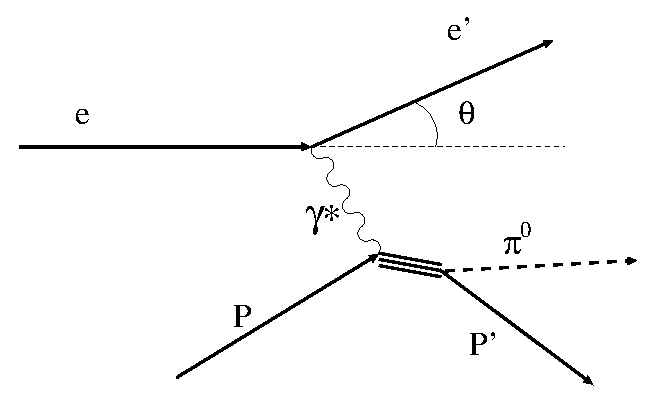
\includegraphics[height=6cm, width = 8cm]{img/cross} 
  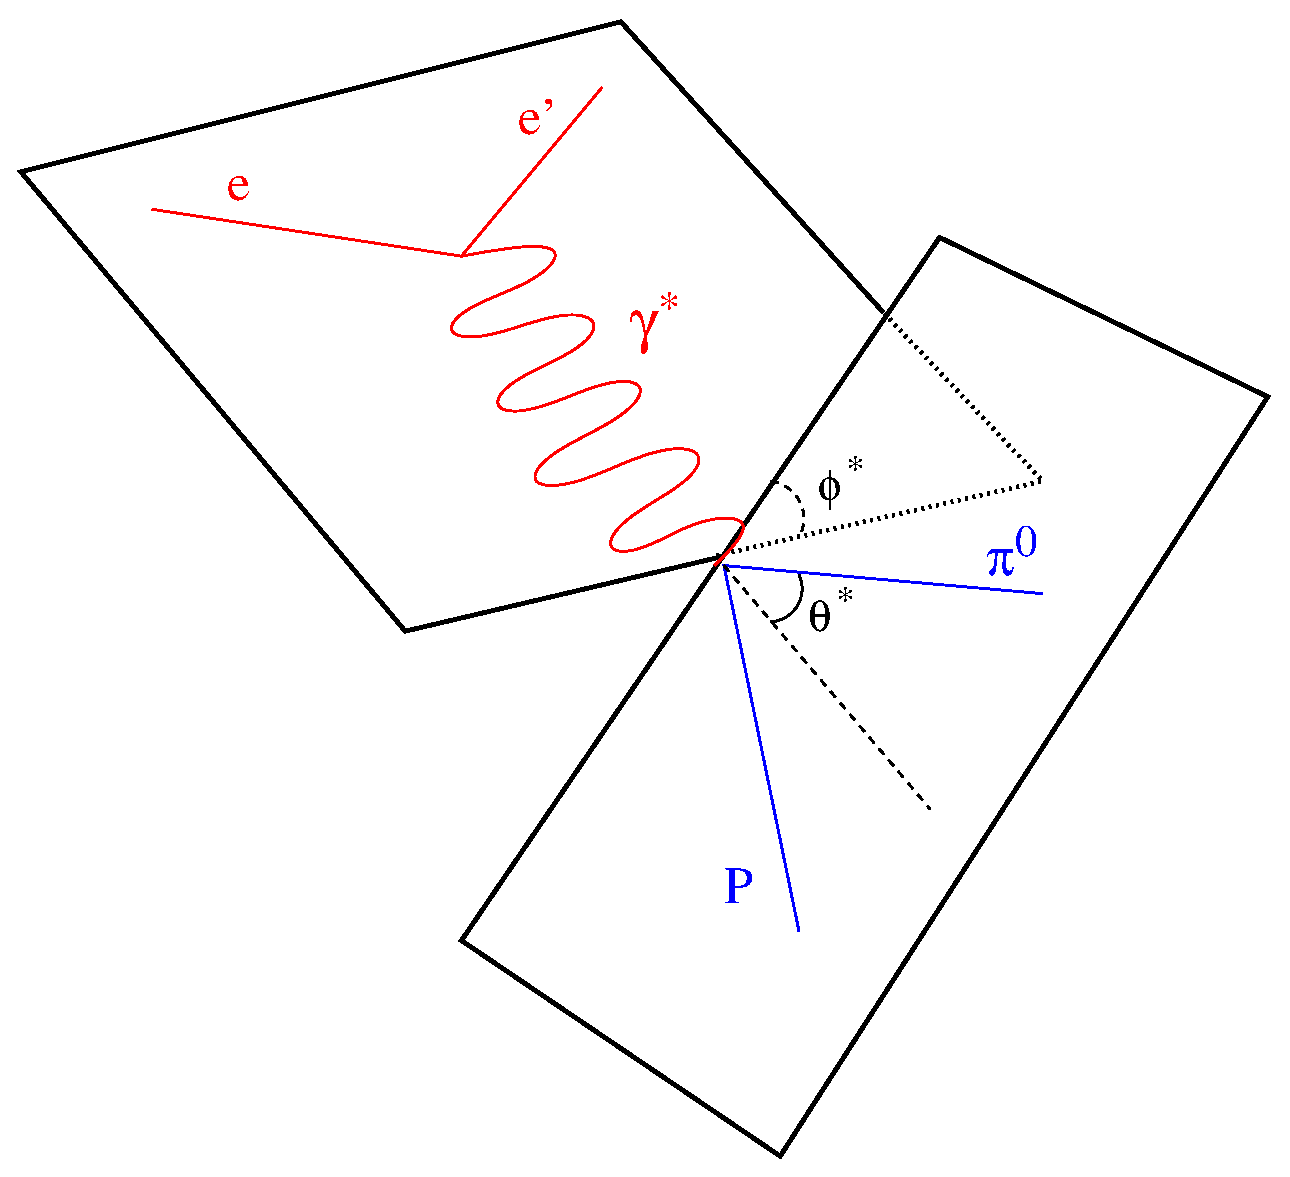
\includegraphics[height=6cm, width = 6cm]{img/kine} 
  \caption{\cit Schematics of  $\pi^0$ electroproduction. On the right the definitions of the angles $\phi^*$ and $\theta^*$.}
  \label{fig:feyn}
 \end{center}
\end{figure}
\vspace{1cm}
can be written as 
$$
 \Dfrac{d\sigma}{dWdQ^{ 2}d\Omega^*_{\pi^0}} = J \Gamma \Dfrac{d\sigma}{d\Omega^*_{\pi^0}}
$$
where $J$ is the Jacobian for the variables transformation $(E_{e'}\, ,\Omega_{e'}) \rightarrow (W\, ,Q^2) $,
$\Gamma $ is the virtual photon flux factor, and $\Dfrac{d\sigma}{d\Omega^*_{\pi^0}}$ is the $\pi^0$ differential
cross section due to virtual photons.

$$ 
\begin{array}{l c l}
J & = & \Dfrac{\partial(W,Q^2)}{\partial(E_{e'},\Omega_{e'})} =  \Dfrac{\pi W}{E_e E_{e'}m_P} \\ 
\\
\Gamma & = & \Dfrac{\alpha}{2\pi^2} \Dfrac{E_e}{E_{e'}} \Dfrac{W^2 - M_P^2}{2M_PQ^2}
\end{array}
$$
For unpolarized beam and target, the center of mass differential cross section $\Dfrac{d\sigma}{d\Omega^*_{\pi^0}}$ 
can be written
$$
\Dfrac{d\sigma}{d\Omega^*_{\pi^0}} = \Dfrac{2W p^*_{\pi^0}}{W^2-m_P^2}\left( \sigma_T + \epsilon\sigma_L
+\epsilon\sigma_{TT}sin^2\theta^*_{\pi^0} cos2\phi^*_{\pi^0} + 
\sigma_{LT}\sqrt{2\epsilon_L(\epsilon+1)}sin\theta^*_{\pi^0} cos\phi^*_{\pi^0} \right)
$$
where $*$ refers to c.m. quantities (i.e. $p^*_{\pi^0}$ is the momentum of $\pi^0$ in the center of mass).

Four structure functions are present: $\sigma_L$ and $\sigma_T$ refer to longitudinal and transverse polarization of the virtual
photon, while $\sigma_{LT}$ and $\sigma_{TT}$ are their inteferences.
These structure function depend on $W$,$Q^2$ and $cos\theta^*_{\pi^0}$. Hence they can be extracted by binning the cross section
in those variables and fitting the $\phi^*_{\pi^0}$ distributions with a function $A+B cos2\phi^*_{\pi^0}  + Ccos\phi^*_{\pi^0} $ 
as will be described in section 9.

\subsection{Multipoles.}
The structure functions above can be generally expressed in terms of six helicity amplitudes \cite{bib:walker}:

$$
\begin{array}{l c l}
\sigma_T & = & 
|H_1|^2+|H_2|^2 + |H_3|^2 + |H_4|^2
\\
\\
\sigma_L & = & 
|H_5|^2+|H_6|^2
\\
\\
\sigma_{TT} & = & 
Re\left(H_2H_3^*-H_1H_4^*\right)
\\
\\
\sigma_{TL} & = & 
Re\left(H_5^*\left(H_1-H_4\right)+H_6^*\left(H_2+H_3\right)\right)
\\
\\
\end{array}
$$
These consist of 11 real quantities (six complex numbers plus 1 constraint).
Even if we can measure the four structure functions, this is not nearly enough
to uniquely determine all the $H$s. Thus additional models and approximation are needed.
Helicity amplitudes can be written in terms of Legendre polynomials $P_l$ and their derivatives 
$P'$ and $P''$ as follows:
$$
\begin{array}{l c l}
H_1 & = & {1\over 2}\sqrt{2}\sin{\theta}\cos{\frac{\theta}{2}}\,
\displaystyle{\sum_{\ell=1}^\infty}\left( B_{\ell+}-B_{(\ell+1)-}\right)
\left( P''_\ell -P''_{\ell+1}\right) \\
\\
H_2 & = & \sqrt{2}\cos{\frac{\theta}{2}}\,
\displaystyle{\sum_{\ell=1}^\infty}\left( A_{\ell+}-A_{(\ell+1)-}\right)
\left( P'_\ell -P'_{\ell+1}\right) \\
\\
H_3 & = & {1\over 2}\sqrt{2}\sin{\theta}\sin{\frac{\theta}{2}}\,
\displaystyle{\sum_{\ell=1}^\infty}\left( B_{\ell+}+B_{(\ell+1)-}\right)
\left( P''_\ell +P''_{\ell+1}\right) \\
\\
H_4 & = & \sqrt{2}\sin{\frac{\theta}{2}}\,
\displaystyle{\sum_{\ell=1}^\infty}\left( A_{\ell+}+A_{(\ell+1)-}\right)
\left( P'_\ell +P'_{\ell+1}\right) \\
\\
H_5 & = & \sqrt{2}\cos{\frac{\theta}{2}}\,
\displaystyle{\sum_{\ell=1}^\infty}\left( C_{\ell+}-C_{(\ell+1)-}\right)
\left( P'_\ell -P'_{\ell+1}\right) \\
\\
H_6 & = & \sqrt{2}\sin{\frac{\theta}{2}}\,
\displaystyle{\sum_{\ell=1}^\infty}\left( C_{\ell+}+C_{(\ell+1)-}\right)
\left( P'_\ell +P'_{\ell+1}\right) \\
\end{array}
$$
where $\theta$ is the pion center of mass production angle.
Here the $A_{\ell\pm}$, $B_{\ell\pm}$, $C_{\ell\pm}$ are called partial wave helicity elements and $\ell\pm$ refers
to a state with pion orbital angular momentun $\ell$ and total angular momentum $J=\ell\pm\frac{1}{2}$.
The amplitudes can be alternately described in a multipole basis \cite{bib:chew} as follows:
$$
\begin{array}{l c l}
M_{\ell+} & = & \frac{1}{2(\ell+1)}\left( 2A_{\ell+}-(\ell+2)B_{\ell+}\right) \\
\\
E_{\ell+} & = & \frac{1}{2(\ell+1)}\left( 2A_{\ell+}+\ell B_{\ell+}\right) \\
\\
M_{\ell+1,-} & = & \frac{1}{2(\ell+1)}\left( 2A_{\ell+1,-}+\ell B_{\ell+1,-}\right) \\
\\
E_{\ell+1,-} & = & \frac{1}{2(\ell+1)}\left( -2A_{\ell+1,-}+(\ell+2)B_{\ell+1,-}\right) \\
\\
S_{\ell+} & = & \frac{1}{\ell+1}\sqrt{\frac{\vec{q}^2}{Q^2}}C_{\ell+}\\
\\
S_{\ell+1,-} & = & -\frac{1}{\ell+1}\sqrt{\frac{\vec{q}^2}{Q^2}}C_{\ell+1,-}\\
\end{array}
$$
where $\vec{q}$ is the 3-momentum of the virtual photon in the c.m. frame.
\subsection{$\Delta(1232)$ production.}
The  $\Delta(1232)$ has $J^P = \frac{3}{2}^+$. From angular momentum conservation we have
$J=\frac{3}{2}=\ell\pm\frac{1}{2}$ hence $\ell=1,2$. But parity conservation requires $P_\Delta = +1 = P_P \times P_{\pi^0}\times(-\ell1)^\ell=(+1)\times(-1)\times(-1)^\ell$
therefore the only contribution to $\Delta(1232)$ production comes from $\ell=1$ and only the $E_{1+}$, $M_{1+}$ and $S_{1+}$ multipoles 
are present.
Other resonance and the non-resonance background contribute with many other multipoles, however 
the $\Delta(1232)$ mass is reasonably 
separated from the next resonances $P_{11}$ and $S_{11}$, and can be isolated from these with missing mass techniques
\footnote{But they cannot be isolated from non-resonant background.}.



\subsection{Goals.}
My thesis consists in measuring the differential cross section
$\Dfrac{d\sigma}{d\Omega^*_{\pi^0}}$ for different $W$, $Q^2$ values and 
in the extraction of the multipoles $M_{1+}$ (proportional to the magnetic transition form factor $G_M^*$ ) and ratios $R_{EM}=E_{1+}/M_{1+}$,
$R_{SM}=S_{1+}/M_{1+}$ in the $Q^2$ range $2\rightarrow 5 \, GeV^2$.
 
The following assumptions are necessary for a model independent extraction:
\begin{itemize}
\item $M_1$ dominance: dropping all terms that don't interfere with $M_{1+}$
\item limited $\ell$: maximum wave number allowed for the $\pi^0 P$ final state. 
in this analysis both $\ell=1$ and $\ell=2$ cases will be retrieved.
\end{itemize} 
A model dependent extraction of the multipoles will be performed using the DMT, Sato-Lee and maid2000 models described in 
section 1.2.

The data will be compared with the results of various competing theoretical 
expectation like the Constituent Quark Model, Perturbative Quantum Chromo Dynamics, Effective Lagrangian
models, and Generalized Parton Distributions.
Results from previous measurements of $R_{EM}$ and  $R_{SM}$ are illustrated below:

\begin{figure}[h]
 \begin{center}
  \includegraphics[height=11cm]{img/ratios.ps} 
  \caption{\cit Previous measurement of $R_{EM}$ and $R_{SM}$ as a function of $Q^2$. CLAS ( $\bullet$)
               data begin at $0.4$ $GeV^2$. Last two points come from Hall-C measurements and presents two different 
               values: the original result and Cole Smith / Kyungseon Joo refit.
               Curves show recent model calculations: chiral quark-soliton (bold solid and dashed, \cite{bib:soli}), dynamical
               pion cloud (solid \cite{bib:dmt2001} and dashed \cite{bib:pion2}), isboar (dotted, \cite{bib:isobar}), relativistic
               quark model(dot-dashed \cite{bib:relati}).
               } 
 \end{center}
\end{figure}



